

\tikzset{every picture/.style={line width=0.75pt}} %set default line width to 0.75pt

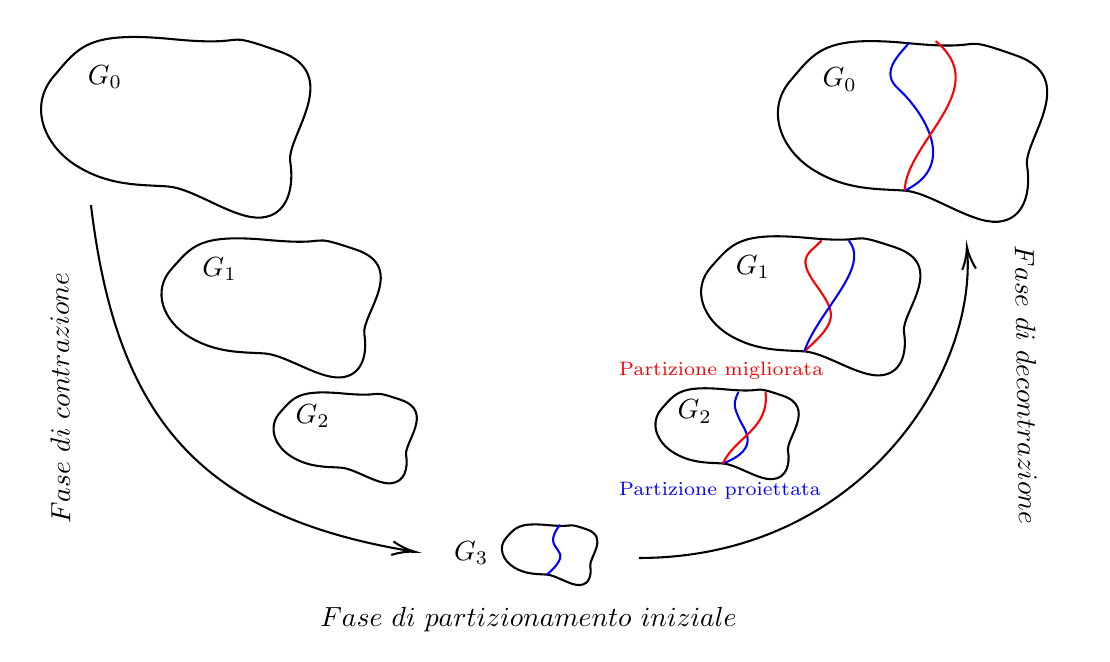
\begin{tikzpicture}[x=0.75pt,y=0.75pt,yscale=-1,xscale=1]
%uncomment if require: \path (0,301); %set diagram left start at 0, and has height of 301

%Shape: Polygon Curved [id:ds5681990127641572]
\draw   (13,23) .. controls (25,9) and (29,1) .. (70,5) .. controls (111,9) and (91,0) .. (122,11) .. controls (153,22) and (125.09,51.89) .. (127,64) .. controls (128.91,76.11) and (126,90) .. (113,91) .. controls (100,92) and (80.66,76.9) .. (68,76) .. controls (55.34,75.1) and (40,76) .. (24,66) .. controls (8,56) and (1,37) .. (13,23) -- cycle ;
%Shape: Polygon Curved [id:ds5791880784550985]
\draw   (69.88,115.65) .. controls (79.65,104.87) and (82.9,98.71) .. (116.29,101.79) .. controls (149.67,104.87) and (133.38,97.94) .. (158.63,106.41) .. controls (183.87,114.88) and (161.14,137.9) .. (162.7,147.22) .. controls (164.25,156.55) and (161.88,167.24) .. (151.3,168.01) .. controls (140.71,168.78) and (124.96,157.16) .. (114.66,156.46) .. controls (104.35,155.77) and (91.86,156.46) .. (78.83,148.76) .. controls (65.81,141.06) and (60.11,126.43) .. (69.88,115.65) -- cycle ;
%Shape: Polygon Curved [id:ds8471099289598505]
\draw   (122.17,184.81) .. controls (128.56,177.76) and (130.68,173.74) .. (152.5,175.75) .. controls (174.32,177.76) and (163.67,173.23) .. (180.17,178.77) .. controls (196.67,184.3) and (181.81,199.34) .. (182.83,205.44) .. controls (183.85,211.53) and (182.3,218.52) .. (175.38,219.02) .. controls (168.46,219.53) and (158.17,211.93) .. (151.44,211.48) .. controls (144.7,211.02) and (136.54,211.48) .. (128.02,206.44) .. controls (119.51,201.41) and (115.79,191.85) .. (122.17,184.81) -- cycle ;
%Shape: Polygon Curved [id:ds042557391147138635]
\draw   (231.1,245.21) .. controls (235.36,240.51) and (236.78,237.83) .. (251.33,239.17) .. controls (265.87,240.51) and (258.78,237.49) .. (269.78,241.19) .. controls (280.78,244.88) and (270.87,254.91) .. (271.55,258.97) .. controls (272.23,263.04) and (271.2,267.7) .. (266.58,268.03) .. controls (261.97,268.37) and (255.11,263.3) .. (250.62,263) .. controls (246.13,262.69) and (240.68,263) .. (235,259.64) .. controls (229.32,256.29) and (226.84,249.91) .. (231.1,245.21) -- cycle ;
%Shape: Polygon Curved [id:ds19971791116540039]
\draw   (368,25) .. controls (380,11) and (384,3) .. (425,7) .. controls (466,11) and (446,2) .. (477,13) .. controls (508,24) and (480.09,53.89) .. (482,66) .. controls (483.91,78.11) and (481,92) .. (468,93) .. controls (455,94) and (435.66,78.9) .. (423,78) .. controls (410.34,77.1) and (395,78) .. (379,68) .. controls (363,58) and (356,39) .. (368,25) -- cycle ;
%Shape: Polygon Curved [id:ds6697871941207159]
\draw   (329.88,114.65) .. controls (339.65,103.87) and (342.9,97.71) .. (376.29,100.79) .. controls (409.67,103.87) and (393.38,96.94) .. (418.63,105.41) .. controls (443.87,113.88) and (421.14,136.9) .. (422.7,146.22) .. controls (424.25,155.55) and (421.88,166.24) .. (411.3,167.01) .. controls (400.71,167.78) and (384.96,156.16) .. (374.66,155.46) .. controls (364.35,154.77) and (351.86,155.46) .. (338.83,147.76) .. controls (325.81,140.06) and (320.11,125.43) .. (329.88,114.65) -- cycle ;
%Shape: Polygon Curved [id:ds6317966254041107]
\draw   (306.17,182.81) .. controls (312.56,175.76) and (314.68,171.74) .. (336.5,173.75) .. controls (358.32,175.76) and (347.67,171.23) .. (364.17,176.77) .. controls (380.67,182.3) and (365.81,197.34) .. (366.83,203.44) .. controls (367.85,209.53) and (366.3,216.52) .. (359.38,217.02) .. controls (352.46,217.53) and (342.17,209.93) .. (335.44,209.48) .. controls (328.7,209.02) and (320.54,209.48) .. (312.02,204.44) .. controls (303.51,199.41) and (299.79,189.85) .. (306.17,182.81) -- cycle ;
%Curve Lines [id:da4556621139317687]
\draw [color={rgb, 255:red, 0; green, 0; blue, 255 }  ,draw opacity=1 ]   (250.62,263) .. controls (267,249) and (246,253) .. (257,239) ;
%Curve Lines [id:da3153745771749539]
\draw [color={rgb, 255:red, 0; green, 0; blue, 255 }  ,draw opacity=1 ]   (335.44,209.48) .. controls (355,202) and (345.05,192.39) .. (343.35,188.03) .. controls (341.65,183.68) and (339.62,181.49) .. (343,175) ;
%Curve Lines [id:da24590148322887484]
\draw [color={rgb, 255:red, 255; green, 0; blue, 0 }  ,draw opacity=1 ]   (335.44,209.48) .. controls (341.44,196.48) and (358,193) .. (356,175) ;
%Curve Lines [id:da8069367964557173]
\draw [color={rgb, 255:red, 255; green, 0; blue, 0 }  ,draw opacity=1 ]   (374.66,155.46) .. controls (391.66,140.46) and (390,137) .. (380,123) .. controls (370,109) and (378,108) .. (383,102) ;
%Curve Lines [id:da030698152549456736]
\draw [color={rgb, 255:red, 0; green, 0; blue, 255 }  ,draw opacity=1 ]   (374.66,155.46) .. controls (381.66,135.46) and (407,115) .. (396,102) ;
%Curve Lines [id:da9188529841976845]
\draw [color={rgb, 255:red, 0; green, 0; blue, 255 }  ,draw opacity=1 ]   (423,78) .. controls (451,65) and (429,37) .. (420,29) .. controls (411,21) and (420,13) .. (425,7) ;
%Curve Lines [id:da500049878186364]
\draw [color={rgb, 255:red, 255; green, 0; blue, 0 }  ,draw opacity=1 ]   (423,78) .. controls (424,54) and (466,29) .. (438,6) ;
%Curve Lines [id:da5337953441131338]
\draw    (31,85) .. controls (42.94,184.5) and (80.62,234.5) .. (185.42,251.74) ;
\draw [shift={(187,252)}, rotate = 189.11] [color={rgb, 255:red, 0; green, 0; blue, 0 }  ][line width=0.75]    (10.93,-3.29) .. controls (6.95,-1.4) and (3.31,-0.3) .. (0,0) .. controls (3.31,0.3) and (6.95,1.4) .. (10.93,3.29)   ;
%Curve Lines [id:da17376352225172775]
\draw    (295,255) .. controls (400.93,255) and (457.86,166.79) .. (453.16,106.81) ;
\draw [shift={(453,105)}, rotate = 84.29] [color={rgb, 255:red, 0; green, 0; blue, 0 }  ][line width=0.75]    (10.93,-3.29) .. controls (6.95,-1.4) and (3.31,-0.3) .. (0,0) .. controls (3.31,0.3) and (6.95,1.4) .. (10.93,3.29)   ;

% Text Node
\draw (28,16.4) node [anchor=north west][inner sep=0.75pt]    {$G_{0}$};
% Text Node
\draw (83.23,108.82) node [anchor=north west][inner sep=0.75pt]    {$G_{1}$};
% Text Node
\draw (128.13,179.36) node [anchor=north west][inner sep=0.75pt]    {$G_{2}$};
% Text Node
\draw (204.41,245.38) node [anchor=north west][inner sep=0.75pt]    {$G_{3}$};
% Text Node
\draw (382,17.4) node [anchor=north west][inner sep=0.75pt]    {$G_{0}$};
% Text Node
\draw (340.23,107.82) node [anchor=north west][inner sep=0.75pt]    {$G_{1}$};
% Text Node
\draw (312.13,177.36) node [anchor=north west][inner sep=0.75pt]    {$G_{2}$};
% Text Node
\draw (10.34,240.07) node [anchor=north west][inner sep=0.75pt]  [rotate=-269.56]  {$Fase\ di\ contrazione$};
% Text Node
\draw (486.92,102.91) node [anchor=north west][inner sep=0.75pt]  [rotate=-89.15]  {$Fase\ di\ decontrazione$};
% Text Node
\draw (140,277.4) node [anchor=north west][inner sep=0.75pt]    {$Fase\ di\ partizionamento\ iniziale$};
% Text Node
\draw (284,217) node [anchor=north west][inner sep=0.75pt]   [align=left] {{\scriptsize \textcolor[rgb]{0,0,1}{Partizione proiettata}}};
% Text Node
\draw (284,159) node [anchor=north west][inner sep=0.75pt]  [font=\normalsize] [align=left] {{\scriptsize \textcolor[rgb]{1,0,0}{Partizione migliorata}}};


\end{tikzpicture}
